%Teori 1/5
%I teorikapitlet skal du plassere din studie inn i et overordnet teoretisk rammeverk. Formålet med dette kapitlet er å gjøre rede for de spesifikke teoriene og begrepene du anvender senere i avhandlingen. Du bør også begrunne hvorfor de er viktige for din studie. Du skal vise at du har forstått teorien du skal anvende. Pass på å bare skrive om det du bruker i analysen eller i tolkningen av datamaterialet.

%Det er verdt å merke seg at ikke alle oppgaver har en egen teoridel. Benytter du deg av IMRoD-modellen, har du presentert tidligere forskning i introduksjonen.

%Dette stoffet skal ha tilknytning til arbeidet som er gjort og gi det bakgrunnsstoffet som er nødvendig for å vurdere resultatene. Kapitlet kan for eksempel omfatte beskrivelse av råvarer/ ingredienser, fremstillingsmetoder, analysemetoder, tidligere arbeider innen temaet, kjemiske ligninger, økonomiske beregninger og sensoriske metoder. Det er ikke nødvendig å ha med mye generelt stoff – lærebokstoff – det kan gi inntrykk av at man ikke behersker emnet man har arbeidet med. 

%NVIDIA’s platforms and application frameworks enable developers to build a wide array of AI applications. Consider potential algorithmic bias when choosing or creating the models being deployed. Work with the model’s developer to ensure that it meets the requirements for the relevant industry and use case; that the necessary instruction and documentation are provided to understand error rates, confidence intervals, and results; and that the model is being used under the conditions and in the manner intended.

\section{Teori}

%Deep learning and unsupervised feature learning have shown great promise in many practical ap- plications. State-of-the-art performance has been reported in several domains, ranging from speech recognition [1, 2], visual object recognition [3, 4], to text processing [5, 6].

%It has also been observed that increasing the scale of deep learning, with respect to the number of training examples, the number of model parameters, or both, can drastically improve ultimate classification accuracy [3, 4, 7]. These results have led to a surge of interest in scaling up the training and inference algorithms used for these models [8] and in improving applicable optimization procedures [7, 9]. The use of GPUs [1, 2, 3, 8] is a significant advance in recent years that makes the training of modestly sized deep networks practical. A known limitation of the GPU approach is that the training speed-up is small when the model does not fit in GPU memory (typically less than 6 gigabytes). To use a GPU effectively, researchers often reduce the size of the data or parameters so that CPU-to-GPU transfers are not a significant bottleneck. While data and parameter reduction work well for small problems (e.g. acoustic modeling for speech recognition), they are less attractive for problems with a large number of examples and dimensions (e.g., high-resolution images).

\subsection{Maskinlæring}

%Over the last several years􏰈 machine learning techniques􏰈 particularly when applied to neural networks􏰈 have played an increasingly imp ortant role in the design of pattern recognition systems􏰇 In fact􏰈 it could be argued that the availability of learning techniques has b een a crucial fac􏰗 tor in the recent success of pattern recognition applications such as continuous speech recognition and handwriting recognition.

\subsubsection{Data is king}
\subsubsection{Datainnsamling}
\subsection{Modell}
\subsubsection{Den biologiske inspirasjonen}
\subsubsection{Bias}
\subsection{Algoritme}
\subsection{Objektdeteksjon}

%Our core visual processing module is a Convolutional Neural Network (CNN) [29, 26], which has emerged as a powerful model for visual recognition tasks [38]. The first application of these models to dense predic- tion tasks was introduced in R-CNN [15], where each re- gion of interest was processed independently. Further work has focused on processing all regions with only single for- ward pass of the CNN [18, 14], and on eliminating explicit region proposal methods by directly predicting the bound- ing boxes either in the image coordinate system [45, 10], or in a fully convolutional [31] and hence position-invariant settings [39, 37, 36]. Most related to our approach is the work of Ren et al. [37] who develop a region proposal net- work (RPN) that regresses from anchors to regions of in- terest. However, they adopt a 4-step optimization process, while our approach does not require training pipelines. Ad- ditionally, we replace their RoI pooling mechanism with a differentiable, spatial soft attention mechanism [20, 17]. In particular, this change allows us to backpropagate through the region proposal network and train the whole model jointly.

\subsection{Trening}
\subsection{Evaluering}
\subsubsection{Nøyaktighet} % error rate
\subsubsection{Presisjon} 
\subsubsection{Konfidensintervall} % confidence interval
\subsection{Inferens}
\subsubsection{Ground truth} %(grunnfestet sanhet?)
\subsubsection{Bilder per sekund} %FPS (bilder per sekund)
\subsubsection{State-of-the-art maskinsyn} % (topp moderne)
\subsubsection{Real-time} %(sanntid)
\subsection{Segmentering}

%Machine Learning: Learning from data
%
%Data is king.
%
%Data collection, annotation, preporation etc.
%
%Data > Algorithm > Training > Evaluation > Deployment > Predictions
%
%	Gather data from every legal source possible (public data sets, purchase data, collect data, synthesize data (super poweful))
%
%	Manually check data
%	Look for biases
%	Look for insights
%	Clean up
%
%	Iterative: Partition data 60 (training)/20 (testing accuracy training)/20 (test)
%
%Model / Algorithm
%
%	Image classification
%	Object detection
%	Segmentation
%
%	Constraints
%
%	Experimentation (test multiple viable models)
%
%Training
%
%	Data augmentation
%	Training parameter (optimizer, rate etc.)
%	Visualizsation (check if it is going correctly)
%
%Evaluation
%
%	Test. Check model size, speed and ACCURACY
%
%Deployment
%
%	Optimizations, deploy, feedback (know when it went badly, check failed images)
%
%\subsection{Build your own}
%
%Build your own:
%
%1) Pick a state-of-the-art architecture
%
%2) Make sure there is an open-source implementation
%
%3) Make sure you get weights for this network trained on ImageNet
%
%
%Experiment
%
%1) Minimal architectural change
%	Fine tune
%
%2) If not enough: Tweak architecture
%	More network blocks, new types of layers etc.
%
%3) Search (Google's neural architecture search)
%
%\subsection{resnet}
%
%\begin{comment}
%ResNet(
%  (conv1): Conv2d(3, 64, kernel_size=(7, 7), stride=(2, 2), padding=(3, 3), bias=False)
%  (bn1): BatchNorm2d(64, eps=1e-05, momentum=0.1, affine=True, track_running_stats=True)
%  (relu): ReLU(inplace=True)
%  (maxpool): MaxPool2d(kernel_size=3, stride=2, padding=1, dilation=1, ceil_mode=False)
%  (layer1): Sequential(
%    (0): Bottleneck(
%      (conv1): Conv2d(64, 64, kernel_size=(1, 1), stride=(1, 1), bias=False)
%      (bn1): BatchNorm2d(64, eps=1e-05, momentum=0.1, affine=True, track_running_stats=True)
%      (conv2): Conv2d(64, 64, kernel_size=(3, 3), stride=(1, 1), padding=(1, 1), bias=False)
%      (bn2): BatchNorm2d(64, eps=1e-05, momentum=0.1, affine=True, track_running_stats=True)
%      (conv3): Conv2d(64, 256, kernel_size=(1, 1), stride=(1, 1), bias=False)
%      (bn3): BatchNorm2d(256, eps=1e-05, momentum=0.1, affine=True, track_running_stats=True)
%      (relu): ReLU(inplace=True)
%      (downsample): Sequential(
%        (0): Conv2d(64, 256, kernel_size=(1, 1), stride=(1, 1), bias=False)
%        (1): BatchNorm2d(256, eps=1e-05, momentum=0.1, affine=True, track_running_stats=True)
%      )
%    )
%    (1): Bottleneck(
%      (conv1): Conv2d(256, 64, kernel_size=(1, 1), stride=(1, 1), bias=False)
%      (bn1): BatchNorm2d(64, eps=1e-05, momentum=0.1, affine=True, track_running_stats=True)
%      (conv2): Conv2d(64, 64, kernel_size=(3, 3), stride=(1, 1), padding=(1, 1), bias=False)
%      (bn2): BatchNorm2d(64, eps=1e-05, momentum=0.1, affine=True, track_running_stats=True)
%      (conv3): Conv2d(64, 256, kernel_size=(1, 1), stride=(1, 1), bias=False)
%      (bn3): BatchNorm2d(256, eps=1e-05, momentum=0.1, affine=True, track_running_stats=True)
%      (relu): ReLU(inplace=True)
%    )
%    (2): Bottleneck(
%      (conv1): Conv2d(256, 64, kernel_size=(1, 1), stride=(1, 1), bias=False)
%      (bn1): BatchNorm2d(64, eps=1e-05, momentum=0.1, affine=True, track_running_stats=True)
%      (conv2): Conv2d(64, 64, kernel_size=(3, 3), stride=(1, 1), padding=(1, 1), bias=False)
%      (bn2): BatchNorm2d(64, eps=1e-05, momentum=0.1, affine=True, track_running_stats=True)
%      (conv3): Conv2d(64, 256, kernel_size=(1, 1), stride=(1, 1), bias=False)
%      (bn3): BatchNorm2d(256, eps=1e-05, momentum=0.1, affine=True, track_running_stats=True)
%      (relu): ReLU(inplace=True)
%    )
%  )
%  (layer2): Sequential(
%    (0): Bottleneck(
%      (conv1): Conv2d(256, 128, kernel_size=(1, 1), stride=(1, 1), bias=False)
%      (bn1): BatchNorm2d(128, eps=1e-05, momentum=0.1, affine=True, track_running_stats=True)
%      (conv2): Conv2d(128, 128, kernel_size=(3, 3), stride=(2, 2), padding=(1, 1), bias=False)
%      (bn2): BatchNorm2d(128, eps=1e-05, momentum=0.1, affine=True, track_running_stats=True)
%      (conv3): Conv2d(128, 512, kernel_size=(1, 1), stride=(1, 1), bias=False)
%      (bn3): BatchNorm2d(512, eps=1e-05, momentum=0.1, affine=True, track_running_stats=True)
%      (relu): ReLU(inplace=True)
%      (downsample): Sequential(
%        (0): Conv2d(256, 512, kernel_size=(1, 1), stride=(2, 2), bias=False)
%        (1): BatchNorm2d(512, eps=1e-05, momentum=0.1, affine=True, track_running_stats=True)
%      )
%    )
%    (1): Bottleneck(
%      (conv1): Conv2d(512, 128, kernel_size=(1, 1), stride=(1, 1), bias=False)
%      (bn1): BatchNorm2d(128, eps=1e-05, momentum=0.1, affine=True, track_running_stats=True)
%      (conv2): Conv2d(128, 128, kernel_size=(3, 3), stride=(1, 1), padding=(1, 1), bias=False)
%      (bn2): BatchNorm2d(128, eps=1e-05, momentum=0.1, affine=True, track_running_stats=True)
%      (conv3): Conv2d(128, 512, kernel_size=(1, 1), stride=(1, 1), bias=False)
%      (bn3): BatchNorm2d(512, eps=1e-05, momentum=0.1, affine=True, track_running_stats=True)
%      (relu): ReLU(inplace=True)
%    )
%    (2): Bottleneck(
%      (conv1): Conv2d(512, 128, kernel_size=(1, 1), stride=(1, 1), bias=False)
%      (bn1): BatchNorm2d(128, eps=1e-05, momentum=0.1, affine=True, track_running_stats=True)
%      (conv2): Conv2d(128, 128, kernel_size=(3, 3), stride=(1, 1), padding=(1, 1), bias=False)
%      (bn2): BatchNorm2d(128, eps=1e-05, momentum=0.1, affine=True, track_running_stats=True)
%      (conv3): Conv2d(128, 512, kernel_size=(1, 1), stride=(1, 1), bias=False)
%      (bn3): BatchNorm2d(512, eps=1e-05, momentum=0.1, affine=True, track_running_stats=True)
%      (relu): ReLU(inplace=True)
%    )
%    (3): Bottleneck(
%      (conv1): Conv2d(512, 128, kernel_size=(1, 1), stride=(1, 1), bias=False)
%      (bn1): BatchNorm2d(128, eps=1e-05, momentum=0.1, affine=True, track_running_stats=True)
%      (conv2): Conv2d(128, 128, kernel_size=(3, 3), stride=(1, 1), padding=(1, 1), bias=False)
%      (bn2): BatchNorm2d(128, eps=1e-05, momentum=0.1, affine=True, track_running_stats=True)
%      (conv3): Conv2d(128, 512, kernel_size=(1, 1), stride=(1, 1), bias=False)
%      (bn3): BatchNorm2d(512, eps=1e-05, momentum=0.1, affine=True, track_running_stats=True)
%      (relu): ReLU(inplace=True)
%    )
%  )
%  (layer3): Sequential(
%    (0): Bottleneck(
%      (conv1): Conv2d(512, 256, kernel_size=(1, 1), stride=(1, 1), bias=False)
%      (bn1): BatchNorm2d(256, eps=1e-05, momentum=0.1, affine=True, track_running_stats=True)
%      (conv2): Conv2d(256, 256, kernel_size=(3, 3), stride=(2, 2), padding=(1, 1), bias=False)
%      (bn2): BatchNorm2d(256, eps=1e-05, momentum=0.1, affine=True, track_running_stats=True)
%      (conv3): Conv2d(256, 1024, kernel_size=(1, 1), stride=(1, 1), bias=False)
%      (bn3): BatchNorm2d(1024, eps=1e-05, momentum=0.1, affine=True, track_running_stats=True)
%      (relu): ReLU(inplace=True)
%      (downsample): Sequential(
%        (0): Conv2d(512, 1024, kernel_size=(1, 1), stride=(2, 2), bias=False)
%        (1): BatchNorm2d(1024, eps=1e-05, momentum=0.1, affine=True, track_running_stats=True)
%      )
%    )
%    (1): Bottleneck(
%      (conv1): Conv2d(1024, 256, kernel_size=(1, 1), stride=(1, 1), bias=False)
%      (bn1): BatchNorm2d(256, eps=1e-05, momentum=0.1, affine=True, track_running_stats=True)
%      (conv2): Conv2d(256, 256, kernel_size=(3, 3), stride=(1, 1), padding=(1, 1), bias=False)
%      (bn2): BatchNorm2d(256, eps=1e-05, momentum=0.1, affine=True, track_running_stats=True)
%      (conv3): Conv2d(256, 1024, kernel_size=(1, 1), stride=(1, 1), bias=False)
%      (bn3): BatchNorm2d(1024, eps=1e-05, momentum=0.1, affine=True, track_running_stats=True)
%      (relu): ReLU(inplace=True)
%    )
%    (2): Bottleneck(
%      (conv1): Conv2d(1024, 256, kernel_size=(1, 1), stride=(1, 1), bias=False)
%      (bn1): BatchNorm2d(256, eps=1e-05, momentum=0.1, affine=True, track_running_stats=True)
%      (conv2): Conv2d(256, 256, kernel_size=(3, 3), stride=(1, 1), padding=(1, 1), bias=False)
%      (bn2): BatchNorm2d(256, eps=1e-05, momentum=0.1, affine=True, track_running_stats=True)
%      (conv3): Conv2d(256, 1024, kernel_size=(1, 1), stride=(1, 1), bias=False)
%      (bn3): BatchNorm2d(1024, eps=1e-05, momentum=0.1, affine=True, track_running_stats=True)
%      (relu): ReLU(inplace=True)
%    )
%    (3): Bottleneck(
%      (conv1): Conv2d(1024, 256, kernel_size=(1, 1), stride=(1, 1), bias=False)
%      (bn1): BatchNorm2d(256, eps=1e-05, momentum=0.1, affine=True, track_running_stats=True)
%      (conv2): Conv2d(256, 256, kernel_size=(3, 3), stride=(1, 1), padding=(1, 1), bias=False)
%      (bn2): BatchNorm2d(256, eps=1e-05, momentum=0.1, affine=True, track_running_stats=True)
%      (conv3): Conv2d(256, 1024, kernel_size=(1, 1), stride=(1, 1), bias=False)
%      (bn3): BatchNorm2d(1024, eps=1e-05, momentum=0.1, affine=True, track_running_stats=True)
%      (relu): ReLU(inplace=True)
%    )
%    (4): Bottleneck(
%      (conv1): Conv2d(1024, 256, kernel_size=(1, 1), stride=(1, 1), bias=False)
%      (bn1): BatchNorm2d(256, eps=1e-05, momentum=0.1, affine=True, track_running_stats=True)
%      (conv2): Conv2d(256, 256, kernel_size=(3, 3), stride=(1, 1), padding=(1, 1), bias=False)
%      (bn2): BatchNorm2d(256, eps=1e-05, momentum=0.1, affine=True, track_running_stats=True)
%      (conv3): Conv2d(256, 1024, kernel_size=(1, 1), stride=(1, 1), bias=False)
%      (bn3): BatchNorm2d(1024, eps=1e-05, momentum=0.1, affine=True, track_running_stats=True)
%      (relu): ReLU(inplace=True)
%    )
%    (5): Bottleneck(
%      (conv1): Conv2d(1024, 256, kernel_size=(1, 1), stride=(1, 1), bias=False)
%      (bn1): BatchNorm2d(256, eps=1e-05, momentum=0.1, affine=True, track_running_stats=True)
%      (conv2): Conv2d(256, 256, kernel_size=(3, 3), stride=(1, 1), padding=(1, 1), bias=False)
%      (bn2): BatchNorm2d(256, eps=1e-05, momentum=0.1, affine=True, track_running_stats=True)
%      (conv3): Conv2d(256, 1024, kernel_size=(1, 1), stride=(1, 1), bias=False)
%      (bn3): BatchNorm2d(1024, eps=1e-05, momentum=0.1, affine=True, track_running_stats=True)
%      (relu): ReLU(inplace=True)
%    )
%  )
%  (layer4): Sequential(
%    (0): Bottleneck(
%      (conv1): Conv2d(1024, 512, kernel_size=(1, 1), stride=(1, 1), bias=False)
%      (bn1): BatchNorm2d(512, eps=1e-05, momentum=0.1, affine=True, track_running_stats=True)
%      (conv2): Conv2d(512, 512, kernel_size=(3, 3), stride=(2, 2), padding=(1, 1), bias=False)
%      (bn2): BatchNorm2d(512, eps=1e-05, momentum=0.1, affine=True, track_running_stats=True)
%      (conv3): Conv2d(512, 2048, kernel_size=(1, 1), stride=(1, 1), bias=False)
%      (bn3): BatchNorm2d(2048, eps=1e-05, momentum=0.1, affine=True, track_running_stats=True)
%      (relu): ReLU(inplace=True)
%      (downsample): Sequential(
%        (0): Conv2d(1024, 2048, kernel_size=(1, 1), stride=(2, 2), bias=False)
%        (1): BatchNorm2d(2048, eps=1e-05, momentum=0.1, affine=True, track_running_stats=True)
%      )
%    )
%    (1): Bottleneck(
%      (conv1): Conv2d(2048, 512, kernel_size=(1, 1), stride=(1, 1), bias=False)
%      (bn1): BatchNorm2d(512, eps=1e-05, momentum=0.1, affine=True, track_running_stats=True)
%      (conv2): Conv2d(512, 512, kernel_size=(3, 3), stride=(1, 1), padding=(1, 1), bias=False)
%      (bn2): BatchNorm2d(512, eps=1e-05, momentum=0.1, affine=True, track_running_stats=True)
%      (conv3): Conv2d(512, 2048, kernel_size=(1, 1), stride=(1, 1), bias=False)
%      (bn3): BatchNorm2d(2048, eps=1e-05, momentum=0.1, affine=True, track_running_stats=True)
%      (relu): ReLU(inplace=True)
%    )
%    (2): Bottleneck(
%      (conv1): Conv2d(2048, 512, kernel_size=(1, 1), stride=(1, 1), bias=False)
%      (bn1): BatchNorm2d(512, eps=1e-05, momentum=0.1, affine=True, track_running_stats=True)
%      (conv2): Conv2d(512, 512, kernel_size=(3, 3), stride=(1, 1), padding=(1, 1), bias=False)
%      (bn2): BatchNorm2d(512, eps=1e-05, momentum=0.1, affine=True, track_running_stats=True)
%      (conv3): Conv2d(512, 2048, kernel_size=(1, 1), stride=(1, 1), bias=False)
%      (bn3): BatchNorm2d(2048, eps=1e-05, momentum=0.1, affine=True, track_running_stats=True)
%      (relu): ReLU(inplace=True)
%    )
%  )
%  (avgpool): AdaptiveAvgPool2d(output_size=(1, 1))
%  (fc): Linear(in_features=2048, out_features=1000, bias=True)
%)
%\end{comment}
%\subsection{Andrej Karpathy}
%
%Andrej Karpathy (5,1 \%)
%
%% Generellt
%
%% Maskinsyn i matindustri
%
%% Mitt arbeid
%
%%Sjømatdivisjonen og Akvadivisjonen ved Nofima har en strategisk internsatsing\footnote{\url{https://nofima.no/prosjekt/sameksistens/}} som går ut på å samle kunnskap om sameksistens mellom ulike marine næringer og interesser, deriblant om hvordan man kan unngå konflikter mellom ulike interesser. 
%
%%En av problemstillingene er sameksistens mellom fiskeri- og oppdrettsnæringene, og hvordan oppdrettsanlegg påvirker de nærliggende fiskeplassene. I den forbindelse er det interessant å kartlegge omfanget av hvitfisk som beiter på fôr fra oppdrettsanlegg. Dette er en problemstilling som har vært i fokus hos media\footnote{For eksempel \url{https://fiskeribladet.no/nyheter/?artikkel=69867} (hentet 12.02.2020)} etter at flere fiskere har fanget fôrsprengt torsk og sei i fjorder hvor det finnes oppdrettsanlegg. Det hevdes at denne fisken er av betydelig dårligere kvalitet og den kan ha fått i seg medisiner gjennom fôret som gjør at den kan være farlig å spise. 
%
%%Det behøves kunnskap om hvor mange villfisk som trekker til oppdrettsanlegg, og under hvilke forhold, slik at man kan komme nærmere en løsning som kan dempe konflikten mellom disse to næringene. 
%
%%\subsection{Mål}
%
%%Målet med dette prosjektet er å utvikle et system som kan telle antall villfisk av ulike arter basert på en videostrøm fra et undervannskamera. Det er ønskelig å kunne vise resultatet som en fordeling av observasjoner over tid for hver art. 
%%Til dette prosjektet er det anskaffet et undervannskamera av typen Steinsvik Orbit-3300 som styres via et MB-3000 kontrollpanel. Dette systemet er utviklet for inspeksjon av fisk i merd og tar opp data i form av en analog videostrøm. Denne kan sendes gjennom en analog-digital-omformer til en datamaskin hvor dataene til slutt vil kunne prosesseres i sanntid. 
%
%%\subsection{Delmål}
%
%%\subsubsection{Programvare skrevet i C++}
%
%%Prosjektet består i hovedsak av å utvikle en programvare som kan gjøre følgende ved hjelp av maskinlæring: 
%
%%\begin{enumerate}
%%\item Segmentere fisk fra bakgrunn
%%\item Klassifisere hver fisk etter art
%%\item Spore hver fisk gjennom hvert bilde i videostrømmen inntil fisken forlater kameraets synsfelt
%%\end{enumerate}
%
%%Programvaren implementeres i C++ ved hjelp av OpenCV-biblioteket\footnote{https://opencv.org/}. Det kan også være aktuelt å lage et grafisk grensesnitt hvor tellingene fra hver art kan vises i sanntid, men dette er avhengig av om prosjektets omfang tillater det. 
%
%%\subsubsection{Praktisk del ved Havbruksstasjonen i Tromsø}
%
%%Det er planlagt en praktisk del hvor kameraet skal plasseres ut på oppdrettsanlegg og samle data som kan prosesseres i ettertid for å teste programvaren. Dette blir mest sannsynlig på Havbruksstasjonen i Tromsø. Å finne beste plasseringen av kameraet i forhold til merdene er en viktig del av dette arbeidet med tanke på synsfelt og lysforhold. 
%
%\subsubsection{Maskinsyn i matindustrien}
%
%Nofima is a research organisation in the food industry
%
%What about the salads and bama
%
%The mathematics course had both calculus and optimization
%
%You can explain about the tedious counting the salad leaves etc
%
%Your data camera may do this
%
%I can justify how computer vision is important in the food industry, and might revolutionize many industries
%
%I can say this is a problem Nofima has, and wanted it solved with computer vision, as it is not only done before it is also cheaper than getting someone to manually count fish.
%
%Say how you came to realise the importance doing practice at Bama, how you tried then to rig up a camera
%
%There are already several players
%
%You have marine robotics
%
%And you have StingRay
%
%The same with marine robotics
%
%They use OpenCV and Qt
%
%Mention that too lakselus very severe problem
%
%I could also mention solving problems in an interesting way is the difference between drudgery and fun
%
%And most problems are solved since they are interesting to someone
%
%%\section{Teori}
%
%\subsubsection{Introduksjon til kunstig intelligens}
%
%Dette er den offisielt første dagen av bacheloroppgaven. Den ble markert med en presentasjon av Sunniva Hoel, der hun presenterte blant annet innsida.ntnu.no/oppgaveskriving og tidligere bacheloroppgaver. Jeg fant en av dem, en litteraturgjennomgang som omhandlet matsvinn, på ntnuopen.ntnu.no.
%
%Jeg avtalte med Stein-Kato på Nofima å møte ham tidlig mandag neste uke. Jeg skal være i Tromsø i to uker og jobbe på oppgaven, i uke 12 og 13.
%
%Jeg har blitt ferdig med det første OpenCV kurset. Jeg har et kurs igjen, som handler om PyTorch, et deep convolutional neural network bibliotek. I løpet av det forrige kurset, lagde jeg en QR-kode leser, jeg lærte om ansiktsgjenkjenning (HAAR algoritmen) og folkemengdegjenkjenning (HOG algoritmen), jeg lagde chroma-keying (greenscreen) og kvisefjerningsprogammer, jeg implementerte algoritmer for noen morfologiske operasjoner som er typisk i maskinsyn fra scratch, jeg implementerte to forskjellige algoritmer som kameraer bruker til autofokus-egenskapen, jeg justerte fargelagene på bilder fra Sergey Prokudin-Gorsky, en klassisk fotograf fra tidlig 1900-tallet, og skal denne uken gjøre ferdig et prosjekt som handler om objektdeteksjon og tracking.
%
%Jeg hadde problemer i går å få tracking, da spesifikt YOLOv3 tracking, til å virke med openCV på windows. I dag fant jeg ut at Visual Studio 2017 (vc15) støttes ikke helt av openCV lenger, og fikk tracking til å virke med Visual Studio 2019 (vc16).
%
%I dag så gjorde jeg ferdig object deteksjon og object tracking prosjektet. Den bruker et dnn som heter YOLOv3, det er en modell som er trent til å gjenkjenne 80 forskjellige objekter. Blant dem er mennesker, bøker, vinglass osv. Det er fascinerende hvor enkelt det er å ta ibruk YOLO, og hvor godt den virker, selv om den ikke er perfekt. For tracking så brukte jeg KFC, en tracker som er implementert i openCV.
%
%OpenCV er kun en inference engine, dvs. den kan kun gjøre "forward passes", eller eksekvere modeller, den kan ikke trene dem. For trening så må jeg ta ibruk PyTorch, som er det neste prosjektet. Ettersom YOLO ikke vet hva en fisk er, og i hvert fall ikke hva en torsk eller sei er, så må jeg trene en dnn selv. Det krever at jeg har mange bilder av fiskene. ImageNet er brukt at dataforskere til å trene netverk, men jeg finner ikke saith eller atlantic cod der. Så jeg får ta noen bilder selv i morgen av fisk fra frysedisken, og håpe at jeg får gode filmer og bilder i Tromsø av sei og torsk.
%
%Jeg skal trene en supervised classification convolution network. Det vil si at jeg vil lære den opp ved å vise mange bilder av det jeg ønsker at den skal kjenne igjen, og noen eksempler på hva som ikke er det den skal vite om. Kunstige neurale nettverk lærer litt som barn. Det er viktig å vise så mange eksempler som mulig, og om en sier at noe er feil så må man være veldig sikker på at det faktisk er feil. Nettverket skal ha 3 outputs. Torsk, sei og ukjent.
%
%Jeg så etter torsk og sei i dag i Trondheim. De selger kun fisk uten hode.
%
%Prosjektet med YOLOv3 modellen må forbedres. Jeg lærte om kaggle.com, den har datasett for dataforskere. Den ser ikke ut til å ha fiskene heller.
%
%Her er planen som alle Machine Learning oppgaver følger, "The ML Pipeline". Den består av følgende
%
%\paragraph{Samling av data:} Kan gjøres på 4 måter.
%
%A) Fra offentlige datasett med lovlige lisenser (kaggle.com, ImageNet osv.)
%B) Kjøpe data
%C) Samle data (Nofima Tromsø)
%D) Syntesere data (Slik som 3D torsken som vi har)
%
%\paragraph{Sjekke data}
%
%A) Manuelt se igjennom dataen (lurt å se alle frames/bilder)
%B) Se etter bias i bildene (f. eks, om bildene av fiskene inkluderer menneskehender, da kan modellen se etter ting på hendene på folk istedet for egenskapene til fisken)
%C) Se etter innsikt (kan lære mye av å bare se på dataen)
%D) Fiks opp dataen
%
%\paragraph{Randomiser dataen}
%
%\paragraph{Partisjoner dataen}
%
%60 \% til trening av modellen
%20 \% til å forbedre modellen (validation)
%20 \% til testing (data modellen har aldri sett før)
%
%Ettersom mennesker er late så er det mer vanlig med denne fordelingen:
%
%80 \% trening
%20 \% validation (test set)
%
%\paragraph{Velg en algoritme eller modell}
%
%Det finnes 3 typer problemer
%
%Image classification
%Object detection
%Segmentation
%
%\paragraph{Tenk på krav}
%
%Presisjon
%Hastighet
%Plattform (mobil, windows, unix, GPU-server, osv.)
%
%\paragraph{Eksperimenter}
%
%Velg en modell, men prøv mange
%
%\paragraph{Valg}
%
%Velg en arkitektur og gjør prosjektet ferdig
%
%I går så ble koronavirus offisielt betegnet som et pandemi av WHO, og Norge ble i dag "stengt". NTNU fraråder reise og campus er stengt for studenter. Stein-Kato har blitt satt i karantene da han har vært i Skottland denne uken. Jeg har avlyst turen til Tromsø. Jeg kommer til å fortsette å trene mine modeller på datasett som er tilgjengelige med PyTorch.
%
%Jeg testet YOLOv3 på en syntetisk 3D torsk som vi har laget, YOLO har aldri sett en fisk før, og trodde det var en fugl. Nå får jeg mer tid på å lære PyTorch, det er egentlig veldig bra at jeg vet mer før jeg lager mitt eget datasett, så vet jeg bedre hva jeg burde gjøre når jeg er i Tromsø.
%
%I dag så skulle jeg egentlig begynne reisen opp til Tromsø, men det ble avlyst pga. koronaviruset. Istedet så har jeg jobbet videre på PyTorch og objekt deteksjon og tracking programmet. Jeg har implementert ReLU, softmax og et kunstig neuron i Python, for å lære mer om hvordan PyTorch virker.
%
%PyTorch er først og fremst rettet mot Python, og forskere og utviklere som foretrekker Python. De har laget et grensesnitt for C++ også. For å forstå PyTorch kreves det en forståelse av kalkulus, også kjent som funksjonsdrøfting, og lineær algebra. Vi hadde om kalkulus i kurset i første året, jeg kan noe lineær algebra fra forkurset, og universitetet jeg gikk på i Skottland.
%
%Et kunstig neuron som anvendes i et neuralt nettverk ligner på ligningen til en linje.
%
%\begin{equation}
%y = ax + b
%\end{equation}
%
%Men den må være for flere dimensjoner.
%
%\begin{equation}
%y = w_i x + b
%\end{equation}
%
%Og X, som er input, kan også bestå av flere dimensjoner. Så en kan like gjerne representere w, weights (lagret i modellen) og input (x) med matriser. b er bias, og må lagres som en vektor.
%
%\begin{equation}
%y = WX + B
%\end{equation}
%
%Og that's it. I python blir dette
%
%\begin{verbatim}
%np.dot(W, X) + B
%\end{verbatim}
%
%Veldig enkelt.
%
%\begin{figure} 
%\begin{center} 
%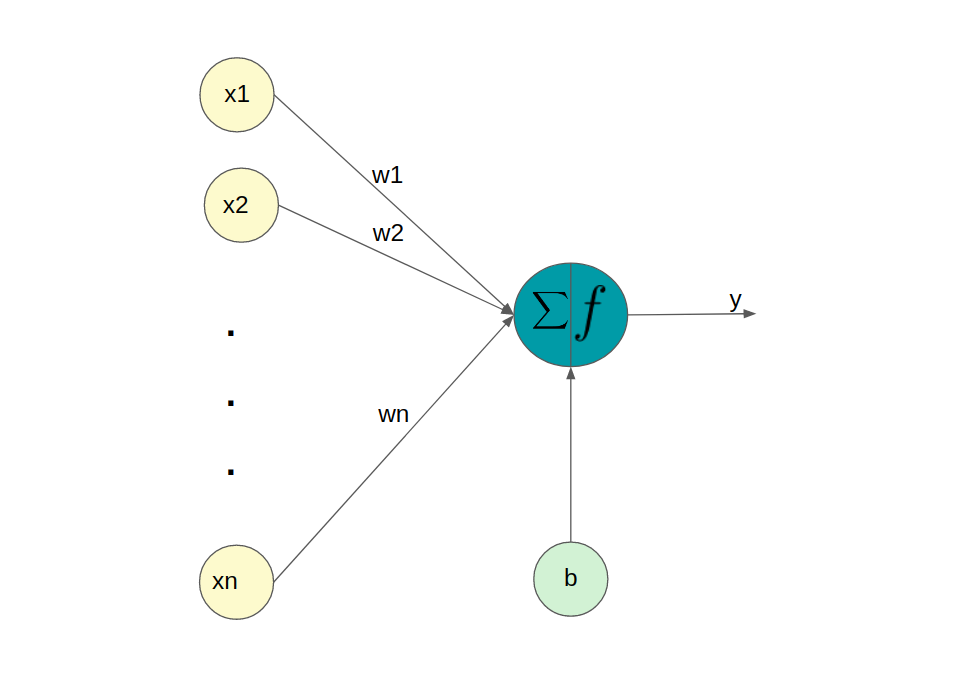
\includegraphics{figures/perceptron}
%\caption{\small \sl Perceptron.\label{fig:perceptron}} 
%\end{center} 
%\end{figure} 
%
%Jeg har implementert stochastic gradient descent i Python + PyTorch. Jeg har også laget nye implementasjoner av softmax, rectifier og kunstige neuroner i PyTorch.
%
%Fordelen med PyTorch er at den er maskinvareakselerert. Det vi si at GPU-en gjør beregningene, ikke bare CPU-en.
%
%GPU-er kommer fra dataspillindustrien. Alle datamaskiner i dag er heterogene, det vil si at de har både en CPU, en generell datahjerne, og en GPU, en grafikkdatahjerne. GPU-er er mange tusen ganger raskere enn en CPU, men kun for oppgaver som er "massively parallel". Både medisin, neurale nettverk, maskinsyn CAD, 3D animasjonsfilmproduksjon, spillutvikling og virtual reality drar nytte fra GPU-er.
%
%Det er viktig i kunstig intelligens å vite hvor et datapunkt hører hjemme. Dette gjøres med kalkulus. Mange av problemene i kunstig intelligens, og maskinsyn, er optimaliseringsproblemer. Stokastic Gradient Descent (SGD) handler om å finne en linje som passer en modell. Det er matematisk optimalisering.
%
%Jeg fikk vite om boken deeplearningboook.org , en gratis og svært god bok om deep learning. Elon Musk sier om boken: "Written by three experts in the field, Deep Learning is the only comprehensive book on the subject." (CEO SpaceX og Tesla)
%
%Jeg har lært mye om deep learning i dag. Jeg har blitt tipset om http://cs231n.stanford.edu/ og http://playground.tensorflow.org/.
%
%Som sagt så er de fleste maskinlæringsproblemer optimaliseringsproblemer. Det handler å finne ut hvor forskjellige datapunkter hører hjemme.
%
%Det finnes flere forskjellige typer problemer. Katogerisering (gi navn på data inn) og regresjon (gi et tall ut fra data inn) er typiske.
%
%Gamle neurale nettverk var perceptrons med lineære aktiveringsfunksjoner der en måtte gjøre features engineering per prosjekt for at modellen skulle virke. En kan leke med dette på tensorflow sin playground, aktiver inputs utover x1 og x2, fjern alle "hidden layers" og sett activation til linear. Test med forskjellig data. Den vil takle dataen som er i to godt avskilte skyer uten at en må tukle med features. Denne gamle måten å trene nettverkene (å finne parametere til activation featuren, for så å lage gode weights for modellen) krevde at en hadde god intuisjon om dataen en ønsket å trene nettverket på. Deep Learning med en ikke-lineær aktiveringsfunksjon gjør at den samme arkitekturen virker for alle problemer, uten feature engineering. Dette kan også lekes med, lag en eller to "hidden layers", fjern alle features untatt x1 og x2, og velg en ikke-lineær aktiveringsfunksjon. Vips, den takler alle data uten noen engineering/tweakkng, gitt nok neuroner. Tensorflow er Google sin rival til PyTorch, PyTorch er laget av Facebook.
%
%PyTorch er delvis implementert i CUDA. Dette er en GPGPU-API som fungerer kun på Nvidia GPU-er. Jeg er mer interessert i Khronos sin OpenCL-standard, som er støttet av AMD, Nvidia, Intel, samt ARM og mange mobile GPU produsenter. Jeg får bruke PC-en i stua, som har en Nvidia-GPU, når jeg trener nettverket med PyTorch.
%
%\begin{figure} 
%\begin{center} 
%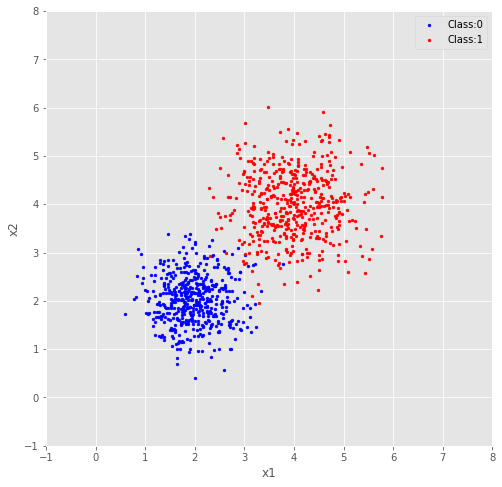
\includegraphics{figures/datapunkter}
%\caption{\small \sl Eksempel av datapunkter. De består av to forskjellige klasser, vist i rødt og blått.\label{fig:datapoints}} 
%\end{center} 
%\end{figure} 
%
%Se figur \ref{datapoints}. 
%
%\begin{figure} 
%\begin{center} 
%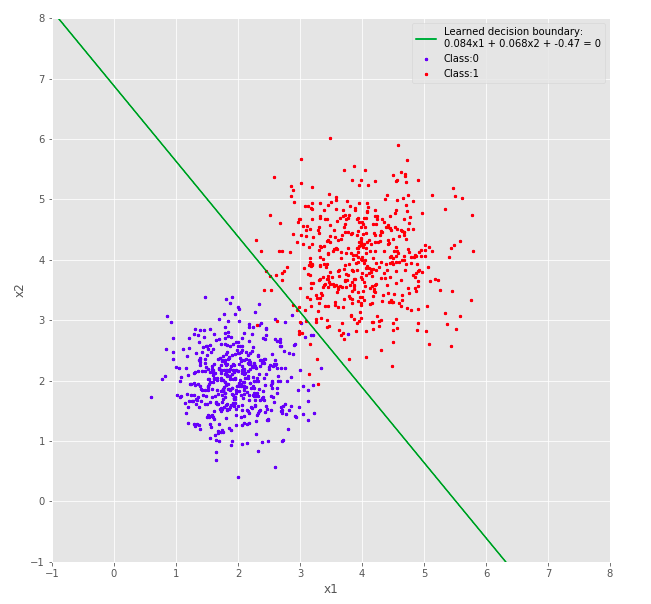
\includegraphics{figures/decision_boundary}
%\caption{\small \sl Figuren over viser decision boundary. Det er dette ML handler om, å lage denne funksjonen som skiller dataen i to grupper, her binært til gruppe 0 og 1.\label{fig:datapoints}} 
%\end{center} 
%\end{figure} 
%
%Jeg har begynt å trene opp en cnn. Jeg har en viss oversikt over deep learning nå. Det var i 2012 deep learning ble stort med AlexNet, de vant ImageNet med stor margin ved å finne på en ny måte å gjøre maskinlæring, det var deep learning.
%
%Jeg har samlet en del whitepapers som jeg skal bruke i rapporten.
%
%PyTorch har mange modeller. De har blitt veldig gode siden 2012, da måtte teamet til Geoffrey Hinton lage hele nettverket selv i CUDA. Nå er det veldig lett å lage programmer som kjenner igjen bilder med PyTorch. PyTorch gjør det også lett å laste ned test-data, og laste inn datasett, til å teste og trene modellen en velger.
%
%Det er visstnok ikke lov ("de vil se stygt på deg") å si at et kunstig neuron er som et biologisk neuron. Det er litt som å si at et fly er som en fugl. Kunstige neuroner er lignende biologiske neuroner på samme måte som fly er inspirert av fugler. 
%
%\begin{figure} 
%\begin{center} 
%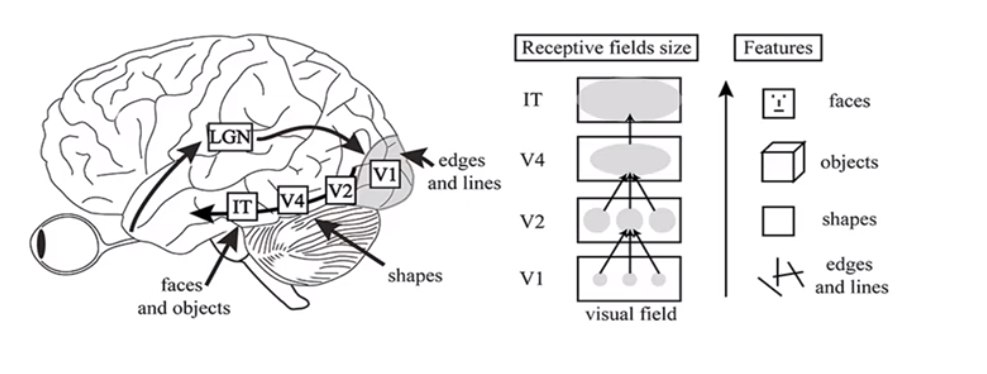
\includegraphics{figures/biological_inspiration_cnn}
%\caption{\small \sl Den biologiske inspirasjonen for cnn.\label{fig:datapoints}} 
%\end{center} 
%\end{figure} 
%
%\begin{figure} 
%\begin{center} 
%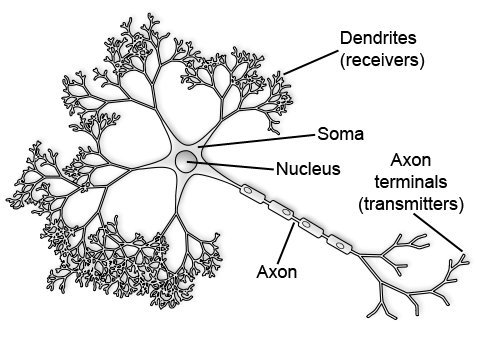
\includegraphics{figures/neuron_figure}
%\caption{\small \sl Neuron\label{fig:datapoints}}
%% https://commons.wikimedia.org/wiki/File:Neuron_figure.png
%% Nicolas.Rougier 
%\end{center} 
%\end{figure} 
%
%I dag trente jeg en ny modell og forbedret den jeg jobbet på Fredag. Denne modellen er trent med data fra PC-en min, av en panda, katt og hund. Det jeg gjorde i dag var bare en test på pipelinen og på at dataen lastes inn riktig. Jeg testet dermed kun 1 % av bildene i datasettet. Jeg fikk allikevel gode resultater. Da kan jeg gå videre.
%
%Jeg fant mange gode whitepapers på deteksjon og tracking av fisk. Å google "fish detection" gir mange resultater fra mange forskjellige prosjekter. Det blir veldig nyttig for senere.
%
%Treningen jeg skal gjøre er å lage en modell som ser forskjellen på torsk og sei. Jeg skal også lage et program som tracker og teller fisken. Å telle fisken er trivielt etter deteksjon. Dette er fine-grained detection. Jeg fant en whitepaper som tar opp spesifikt å detektere fisk av forskjellige fiskearter. Kanskje jeg låner ideer fra dem. Kan også prøve å trene deres datasett også for å få litt mer erfaring.
%
%https://www.kaggle.com/ashishsaxena2209/animal-image-datasetdog-cat-and-panda
%
%\url{https://www.researchgate.net/publication/317558591_Automatic_fish_species_classification_in_underwater_videos_Exploiting_pretrained_deep_neural_network_models_to_compensate_for_limited_labelled_data}
%
%Steg 1 - Forstå problemet
%Steg 2A - Få tak i data
%Steg 2B - Utforsk og forstå dataen
%Steg 2C - Lag et utvalg av dataen fra datasettet
%Steg 3 - Gjør klar dataen
%Steg 4 - Tren en enkel modell på datautvalget og test pipelinen før trening av et komplett nettverk påbegynnes
%Steg 5 - Tren med et komplett datasett
%Steg 6 - Iterativt forbedre modellen
%
%I dag jobbet jeg på modellen. Jeg har testet den på datasei og datatorsk. Den klarer å se forskjellen på dem med 100 \% nøyaktighet. Jeg har enda ikke gjort ferdig modellen. Jeg må fortsatt trene hele modellen, så langt så har jeg gjort steg 1-4, jeg har steg 5-6 igjen. Den neste delen av oppgaven blir å bruke modellen til objekt deteksjon og tracking i en film, slik jeg gjorde med YOLOv3 modellen tidligere.
%
%Jeg skal lage et nytt datasett med ekte torsk og sei.
%
%\begin{figure} 
%\begin{center} 
%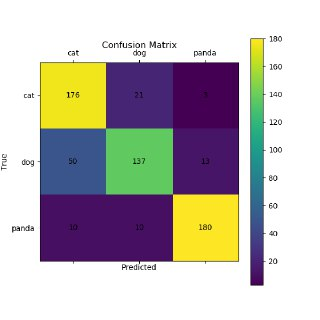
\includegraphics{figures/confusion_matrix}
%\caption{\small \sl Forvirringsmatrise. n*n. Den vil vise falske positive, sanne positive, falske negative og sanne negative for hver klasse. Om denne cnn-en var for å detektere brystkreft, og positivt sykdom betyr at en kvinne har brystkreft, så hadde falske positive vært ganske dårlig, og falske negative vært katastrofalt. En modell som, for eksempel, sier negativ hele tiden vil være 95 \% riktig, da bryskreft skjer sjeldent (i 5 \% av tilfellene, i dette tilfellet). Bias er farlig, det er viktig å balansere dataen sendt til en modell. Like mye data per klasse. \label{fig:datapoints}}
%\end{center} 
%\end{figure} 
%
%I dag implementerte jeg step-wise learning decay til modellen i et forsøk på å få bedre nøyaktighet. En modell skal ha høy learning rate i begynnelsen, så skal den bli mindre for å nå bunnen av læringskurven.
%
%Videre, å detektere fisk med maskinsyn har blitt gjort før. Det er mye bra som er skrevet om dette.
%
%Vi diskuterte hva som har gjort deep learning så populært den siste tiden. Her er nye fremskritt de siste 10 årene som har gjort deep learning populært (LeNet vs AlexNet, Andrej Karpathy 2020)
%
%\begin{figure} 
%\begin{center} 
%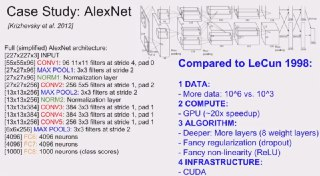
\includegraphics{figures/alexnet}
%\caption{\small \sl Vi diskuterte hva som har gjort deep learning så populært den siste tiden. Her er nye fremskritt de siste 10 årene som har gjort deep learning populært (LeNet vs AlexNet, Andrej Karpathy 2020) \label{fig:datapoints}}
%\end{center} 
%\end{figure} 
%
%Jeg har fått til YOLOv3 nå. Den går mye raskere enn RetinaNet, og kan gå i sanntid med en Nvidia GPU, slik som en 2070 gtx (regner jeg med).
%
%Jeg har brukt dagen på å se på tracking. Den må tracke flere objekter, det betyr flere trackere. En tracker krever ganske mye fra CPU-en. Det gjør programmet saktere. Men de kan multithreades. Jeg har enda ikke klart å gjøre alle fiskene som blir detektert til noe som trackes. Tracking skal være raskere enn objektdeteksjon. Jeg kan gjøre deteksjon sjeldnere enn tracking, slik at programmet går raskere. Men det må fortsatt testes. Deteksjon må uansett skje med jevne mellomrom, da nye kommer stadig inn i i bildet.
%
%Jeg har laget flere masks for segmentering, som blir et siste eksperiment, etter YOLOv3 er trent opp på sei og tracking er blitt eksperimentert med.
%
%Jeg snakket med Nofima i dag. Jeg forklarte arbeidet som jeg har gjort. Vi ble enige om å se litt mer på tracking, jeg forklarte at deteksjon uten tracking vil nok virke like bra.
%
%I dag lastet jeg opp realeases av app på github. Stein-Kato har tilgang til prosjektet nå. Jeg håper han får brukt arbeidet.
%
%Jeg har begynt å se på segmentering. Jeg håper å bli med på to kaggle konkurranser i løpet av måneden. Jeg har begynt å tenke mer på rapporten, skrivingen får nesten begynne for fullt nå, så stiller jeg bedre forberedt til BO-seminaret den 30. April.
%
%\subsubsection{Maskinlæring}
%
%Machine Learning: Learning from data
%
%Data is king.
%
%Data collection, annotation, preporation etc.
%
%Data > Algorithm > Training > Evaluation > Deployment > Predictions
%
%	Gather data from every legal source possible (public data sets, purchase data, collect data, synthesize data (super poweful))
%
%	Manually check data
%	Look for biases
%	Look for insights
%	Clean up
%
%	Iterative: Partition data 60 (training)/20 (testing accuracy training)/20 (test)
%
%Model / Algorithm
%
%	Image classification
%	Object detection 
%	Segmentation
%
%	Constraints
%
%	Experimentation (test multiple viable models)
%
%Training
%
%	Data augmentation
%	Training parameter (optimizer, rate etc.)
%	Visualizsation (check if it is going correctly)
%
%Evaluation
%	
%	Test. Check model size, speed and ACCURACY
%
%Deployment
%
%	Optimizations, deploy, feedback (know when it went badly, check failed images)	
%
%\subsubsection{Neural networks}
%
%Classification (Supervised learning)
%
%	Seperating data into groups
%
%	Binary classification (two groups) (Sigmoid activation is used)
%
%	Multiclass classification (Activation: Softmax) (Loss function: Cross entropy loss)
%
%	Regression (Activation: Linear) (Loss function: MSE loss)
%
%	Decision boundary seperates the groups by the decision function
%
%	Training is learning the decision function
%
%	Deciding decision function is called training
%
%	Data is on a plane (2D) or a hyperplane (higher dimensions)
%
%	Input layer > Hidden layer (can be many layers) > output
%
%	Each layer (node) in a nn is a neuron or perceptron
%
%	Perceptron: Calculate weighted sum of inputs and add bias. Then apply activation function (non-linear)
%
%	Every layer looks for a pattern found in the previous layer. If it is found, it "fires up"
%
%	An example of an activation function is ReLU (Rectified Linear Unit)
%
%	Another example is the sigmoid function, and tanh
%
%	An activation function creates non-linearity
%
%	The number of hidden layers is called the networks depth (depth = 2 is typical for simple problems)
%
%Loss functions
%
%	Classification outputs a category (class)
%
%	Regression outputs numerical values (or a vector of numerical values)
%
%	Many problems are optimizatino problems in ML, either to minimize or maximaze a value of a function
%
%	These functions are called the objective function
%
%	When finding the minimum, it is called a loss, or cost, function
%
%	e = y - \^y (error is ground thruth minus model output)
%
%	An error, L, can be considered either a square (MSE, most common) or an absolute number (MAE, when data has many outliers)
%
%Single layer perceptron kan løse lineære problemer
%
%Ved å gjøre "feature engineering" så kan ikke-lineære problemer løses
%
%Deep learning gjør at en kan løse lineære problemer om en bruker ikke-lineær aktivering. ReLU konvergerer raskt.
%
%%\subsubsection{Maskinsyn med OpenCV}
%%\subsubsection{Video med undervannskamera fra merdene}
%%\subsubsection{Analysere video}
%%\subsubsection{Deep Learning med OpenCV}
%%\subsubsection{PyTorch}
%%\subsubsection{Segmentere ut fisk}
%%\subsubsection{Object Detection med OpenCV}
%%\subsubsection{Object Tracking med OpenCV}
%%\subsubsection{Klassifisere hver fisk etter art}
%%\subsubsection{Registrere antall individer av hver art fortløpende}
%%\subsection{Praktisk gjennomføring}
%%\subsubsection{Programvareutvikling med maskinlæring implementert i C++}
%%\subsubsection{Videostrøm fra merdene}
%%\subsection{Resultater}
%%\subsection{Diskusjon}
%%\subsection{Konklusjon}
%%\subsection{Referanseliste}
